% allgem. Dokumentenformat
\documentclass[a4paper,12pt,headsepline]{scrartcl}
%Variablen welche innerhalb der gesamten Arbeit zur Verfügung stehen sollen
\newcommand{\titleDocument}{Bachelor- / Masterarbeit}
\newcommand{\subjectDocument}{im Studiengang <Studiengang>}

% weitere Pakete
% Grafiken aus PNG Dateien einbinden
\usepackage{graphicx}
\usepackage{scrextend}
\usepackage{gensymb}
\usepackage[numbers]{natbib}
\graphicspath{ {./img/procedure/}{./img/results/}{./img/intro/}{./img/task/}{./img/procedure/}} 

% Eurozeichen einbinden
\usepackage[right]{eurosym}

% Umlaute unter UTF8 nutzen
\usepackage[utf8]{inputenc}

% Zeichenencoding
\usepackage[T1]{fontenc}

\usepackage{lmodern}
\usepackage{fix-cm}

% floatende Bilder ermöglichen
%\usepackage{floatflt}

% mehrseitige Tabellen ermöglichen
\usepackage{longtable}

% Unterstützung für Schriftarten
%\newcommand{\changefont}[3]{ 
%\fontfamily{#1} \fontseries{#2} \fontshape{#3} \selectfont}

% Packet für Seitenrandabständex und Einstellung für Seitenränder
\usepackage{geometry}
\geometry{left=3.5cm, right=2cm, top=2.5cm, bottom=2cm}

% Paket für Boxen im Text
\usepackage{fancybox}

% bricht lange URLs "schoen" um
\usepackage[hyphens,obeyspaces,spaces]{url}

% Paket für Textfarben
\usepackage{color}

% Mathematische Symbole importieren
\usepackage{amssymb}

% auf jeder Seite eine Überschrift (alt, zentriert)
%\pagestyle{headings}

% erzeugt Inhaltsverzeichnis mit Querverweisen zu den Kapiteln (PDF Version)
\usepackage[bookmarksnumbered,pdftitle={\titleDocument},hyperfootnotes=false]{hyperref} 
%\hypersetup{colorlinks, citecolor=red, linkcolor=blue, urlcolor=black}
%\hypersetup{colorlinks, citecolor=black, linkcolor= black, urlcolor=black}

% neue Kopfzeilen mit fancypaket
\usepackage{fancyhdr} %Paket laden
\pagestyle{fancy} %eigener Seitenstil
\fancyhf{} %alle Kopf- und Fußzeilenfelder bereinigen
\fancyhead[L]{\nouppercase{\leftmark}} %Kopfzeile links
\fancyhead[C]{} %zentrierte Kopfzeile
\fancyhead[R]{\thepage} %Kopfzeile rechts
\renewcommand{\headrulewidth}{0.4pt} %obere Trennlinie
%\fancyfoot[C]{\thepage} %Seitennummer
%\renewcommand{\footrulewidth}{0.4pt} %untere Trennlinie

% für Tabellen
\usepackage{array}

% Runde Klammern für Zitate
%\usepackage[numbers,round]{natbib}

% Festlegung Art der Zitierung - Havardmethode: Abkuerzung Autor + Jahr

% Schaltet den zusätzlichen Zwischenraum ab, den LaTeX normalerweise nach einem Satzzeichen einfügt.
\frenchspacing

% Paket für Zeilenabstand
\usepackage{setspace}

% für Bildbezeichner
\usepackage{capt-of}

% für Stichwortverzeichnis
\usepackage{makeidx}

% für Listings
\usepackage{listings}
\lstset{numbers=left, numberstyle=\tiny, numbersep=5pt, keywordstyle=\color{black}\bfseries, stringstyle=\ttfamily,showstringspaces=false,basicstyle=\footnotesize,captionpos=b}
\lstset{language=java}

% Indexerstellung
\makeindex

% Abkürzungsverzeichnis
\usepackage[german]{nomencl}
\let\abbrev\nomenclature

% Abkürzungsverzeichnis LiveTex Version
\renewcommand{\nomname}{Abkürzungsverzeichnis}
\setlength{\nomlabelwidth}{.25\hsize}
\renewcommand{\nomlabel}[1]{#1 \dotfill}
\setlength{\nomitemsep}{-\parsep}
\makenomenclature
%\makeglossary

% Abkürzungsverzeichnis TeTEX Version
% \usepackage[german]{nomencl}
% \makenomenclature
% %\makeglossary
% \renewcommand{\nomname}{Abkürzungsverzeichnis}
% \setlength{\nomlabelwidth}{.25\hsize}
% \renewcommand{\nomlabel}[1]{#1 \dotfill}
% \setlength{\nomitemsep}{-\parsep}

% Disable single lines at the start of a paragraph (Schusterjungen)
\clubpenalty = 10000
% Disable single lines at the end of a paragraph (Hurenkinder)
\widowpenalty = 10000
\displaywidowpenalty = 10000

\begin{document}
% hier werden die Trennvorschläge inkludiert
%hier müssen alle Wörter rein, welche Latex von sich auch nicht korrekt trennt bzw. bei denen man die genaue Trennung vorgeben möchte
\hyphenation{
Film-pro-du-zen-ten
Lux-em-burg
Soft-ware-bau-steins
zeit-in-ten-siv
}

%Schriftart Helvetica
%\changefont{phv}{m}{n}


% Titelseite %
% das Papierformat zuerst
%\documentclass[a4paper, 11pt]{article}

% deutsche Silbentrennung
%\usepackage[ngerman]{babel}

% wegen deutschen Umlauten
%\usepackage[ansinew]{inputenc}

% hier beginnt das Dokument
%\begin{document}


\thispagestyle{empty}

%\begin{figure}[t]
% \includegraphics[width=0.6\textwidth]{abb/fh_koeln_logo}
%\end{figure}


\begin{verbatim}


\end{verbatim}

\begin{center}
\Large{Universität Tübingen}\\
\Large{- Mathematisch-Naturwissenschaftliche Fakultät -}\\
\end{center}


\begin{center}
\Large{Masterarbeit}
\end{center}
\begin{verbatim}




\end{verbatim}
\begin{center}
\doublespacing
\textbf{\LARGE{Spatial problem solving and collaboration in virtual reality}}\\
\singlespacing
\begin{verbatim}

\end{verbatim}
\textbf{im Studiengang Kognitionswissenschaft}
\end{center}
\begin{verbatim}

\end{verbatim}
\begin{center}

\end{center}
\begin{verbatim}

\end{verbatim}
\begin{center}
\textbf{zur Erlangung des akademischen Grades Master of Science}
\end{center}
\begin{verbatim}






\end{verbatim}
\begin{flushleft}
\begin{tabular}{llll}
\textbf{Autor:} & & Marcel Bechtold& \\
& & MatNr. 3949100 & \\
& & \\
\textbf{Version vom:} & & \today &\\
& & \\
\textbf{1. Betreuerin:} & & Prof. Dr. Enkelejda Kasneci &\\
\textbf{2. Betreuer:} & & Dr. Tobias Meillinger &\\
\end{tabular}
\end{flushleft}

% römische Numerierung
%\pagenumbering{arabic}

% 1.5 facher Zeilenabstand
\onehalfspacing

% einfacher Zeilenabstand
\singlespacing

% Inhaltsverzeichnis anzeigen
\newpage
\tableofcontents

\newpage

% das Abbildungsverzeichnis
%\newpage
% Abbildungsverzeichnis soll im Inhaltsverzeichnis auftauchen
\addcontentsline{toc}{section}{List of Figures}
% Abbildungsverzeichnis endgueltig anzeigen
\listoffigures

% das Tabellenverzeichnis
%\newpage
% Abbildungsverzeichnis soll im Inhaltsverzeichnis auftauchen
\addcontentsline{toc}{section}{List of Tables}
% \fancyhead[L]{Abbildungsverzeichnis / Abkürzungsverzeichnis} %Kopfzeile links
% Abbildungsverzeichnis endgueltig anzeigen
\listoftables

% Definiert Stegbreite bei zweispaltigem Layout
\setlength{\columnsep}{25pt}

%%%%%%% EINLEITUNG %%%%%%%%%%%%
%\twocolumn
\newpage
\fancyhead[L]{\nouppercase{\leftmark}} %Kopfzeile links

% 1,5 facher Zeilenabstand
\onehalfspacing

% einzelne Kapitel
\newpage
\section{Introduction} \label{sec:introduction}

Problem solving is a meanwhile well established field in cognitive psychology. Generally problem solving can be described as the search within a problem space. \cite{Newell1972}. The literature suggests that different sub processes of problem solving need to be considered in order to understand the whole process. The relevant sub-processes are the perception of the task, understanding the problem, activating foreknowledge, manipulating the given information, dividing the problem into subgoals, developing a plan, detecting errors and finding and validating results. The sub-processes of problem solving can also be investigated separately. Problem solving can also be defined by the attempt to transition from a given initial state to a goal state. Furthermore it is necessary that there must be some kind of barrier that does not allow to achieving the goal state directly. \cite{muesseler2015allgemeine}

In previous research some common methods of investigating problem solving have been established. The main goal is to identify the cognitive and neuronal processes of problem solving. A popular method is eye tracking because it allows to identify which informations of a problem are being looked at and also gives information about action planning. \cite{underwood2005}  Furthermore, neuropsychological studies are used to investigate which brain areas are responsible for certain aspects of problem solving. \cite{Karnath2006} In general there already are several tasks which are being used to investigate problem solving in behavioral studies. One example is the nine dot problem. The problem is to connect all nine dots of a 3x3 matrix with four continuous straight lines and without taking the pen of the paper (see Figure \ref{fig:ninedots}).

\begin{figure}[h]
\centering
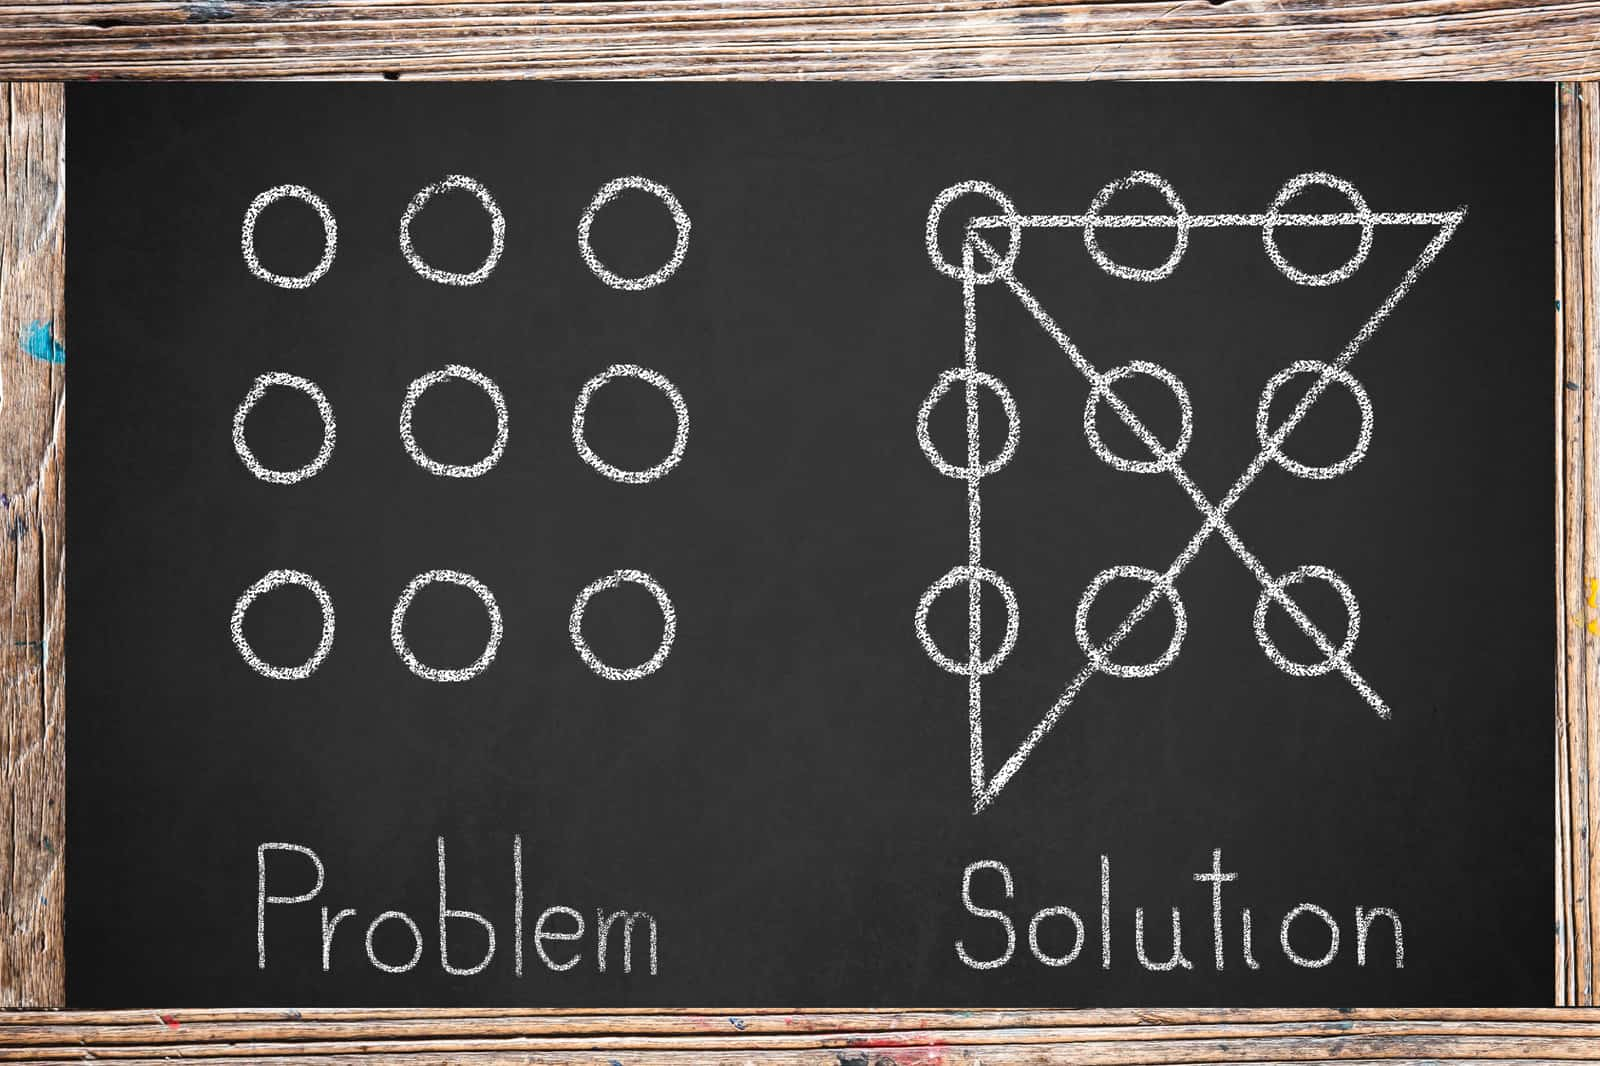
\includegraphics[width=0.5\textwidth]{ninedots}
\caption{Solution of the nine dot problem.}
\label{fig:ninedots}
\end{figure}

\newpage

In contrast to the more general approaches of problem solving described before, this work focuses on spatial problem solving and the question whether two people together perform better than a single person in a spatial problem solving task. 
Previous work in spatial problem solving has targeted fundamental processes of how individuals apply spatial learning, memory and planning. \cite{Waller2013} There also exist studies that investigate collaborative learning, but they do not focus on spatial problems. (e.g.  \cite{Dillenbourg1999} \cite{Hesse2015}) Therefore the main goal of this work is to investigate the combination of spatial and collaborative problem solving.  

Since it is quite difficult to investigate and measure performance in collaborative spatial problem solving tasks in the real world a new task in virtual reality has been designed for this study. This task has been designed in a way that allows to investigate and compare problem solving performance both in individuals and in groups of two. The main benefit of using virtual reality to investigate spatial problem solving is the fact that the technical equipment allows to easily record data of how participants interact with the virtual environment (e.g. controller movements and rotations). Furthermore in a virtual environment the task, the position of participants and the environmental aspects of the scene can be easily manipulated and controlled. Therefore, virtual reality appears to be a very promising method to investigate collaborative spatial problem solving. 

Only very few studies that compare to this approach of this study can be found. One example is the study by Heldal et al. from 2005. \cite{heldal2005}
The purpose of the study was to investigate differences in interfaces solving a virtual reality task similar to the Rubik's Cube like problem presented in this study. An example of the virtual scene that they used can be seen in Figure \ref{fig:heldal}. It has been shown that head mounted displays are one of the best interfaces to investigate spatial problem solving. Since then technology has rapidly developed and there are now much better interfaces and computer graphics available in order to create immersive virtual environments that allow interactions with different kinds of user input.

\begin{figure}[h]
\centering
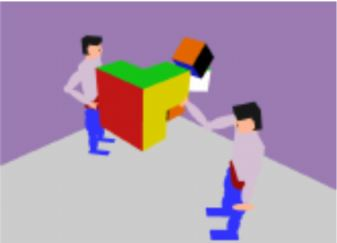
\includegraphics[width=0.5\textwidth]{heldal}
\caption{Virtual scene of the study by Heldal et al. from 2005. \cite{heldal2005}.}
\label{fig:heldal}
\end{figure}

 The main goal of this study was to design a task in a virtual environment that is suitable to investigate and quantify the performance in problem solving both in individuals and groups of two people and also compare both variations.
\newpage
\section{Task Design}

In this section the design and idea behind the task which was used in the experiment will be explained. It is intended to focus on the task design only without considering the virtual reality aspects and and actual procedure which will be described in the methods sections. But is has to be kept in mind that the task is intended to be implemented in a 3D virtual environment which allows participants to almost freely interact and move. The challenge of designing a problem for a spatial problem solving experiment in a virtual 3D space is to find a balance between limiting the options and degrees of freedom participants have, but also allowing them enough possibilities to apply individual strategies within those limitations.

When designing a task (or problem) for a problem solving experiment it is important to think about the complexity of the task. The literature differentiates between simple and complex problems. \cite{muesseler2015allgemeine}  A simple problem is characterized by having a clear initial  and goal state and all transitions and solution paths are known. Such problems suit very well to investigate heuristics, search processes and systematic errors in problem solving. The main advantage is that simple problems can be investigated well in experiments because they can be easily controlled. A complex problem is mainly characterized by the fact that it is more closely related to real life problems, which makes them harder to simulate in an experiment. It is important to understand that a simple problem must not necessearily be easy to solve. The adjective "simple" refers only to the fact that the problem's rules and its scope are limited to a few actions. The nine dot problem described before (Section \ref{sec:introduction} and Figure \ref{fig:ninedots}) can be categorized as a simple problem, because it is only possible to draw straight lines and it is not allowed to take the pen off the paper. Finding the solution still seems to be very difficult since only 10\% of the participants are able to solve the problem. \cite{muesseler2015allgemeine} 
Since we want to be able to quantify and compare performances of individuals and groups of two, the main requirement for the task  was that it is designed to have the characteristics of a simple problem. However, problem solving tasks in the 3D space are naturally pretty complex, because they allow all kinds of different movements and interactions. In the following the task components and rules will be described. Furthermore the theories behind this task will be explained to show why it suits to investigate and compare spatial problem solving for both individuals and groups of two.

\newpage

\subsection{Task components and goal} \label{sec:task_components}
In this section the task components, the initial state and the goal state will be described.
The components of the task are 10 cubes and a solution space with 4 slots to hold one cube each. Every cube has a color on each of its 6 faces. The same color can be assigned at most to two faces of a cube. Since the colors vary in each trial, a digit coding will be introduced in the following to describe the exact color configurations of all cubes. A color configuration of a cube consists of a mapping of all its faces to a digit code. Every digit code is a placeholder for a certain color. An example coding for one cube could look like this: 

\begin{center}
\textbf{front=1, back=0, left=2, right=0, top=7, bottom=8}
\end{center}


The cube faces can have 9 different colors and therefore a digit coding has been defined that ranges from 0 to 8. The 9 different colors are required because the distractor cubes need to be colored with some distractor colors, which are not part of the goal state. Since the resulting cuboid has 6 faces there are 6 colors which are actually part of the goal state. The other 3 colors are the distractor colors. The complete digit coding for all 9 cubes can be found in Table \ref{tab:digit_coding}.

\begin{table}
\begin{center}
    \begin{tabular}{| l | | l | l | l | l | l | l |  l |}
    \hline
    \textbf{Cube} & \textbf{front} & \textbf{back} & \textbf{left} & \textbf{right} & \textbf{top} & \textbf{bottom} & \textbf{type} \\ \hline
    A & 1 & 0 & 2 & 0 & 7 & 8 & starting/solution \\ \hline
    B & 0 & 3 & 2 & 0 & 7 & 8 & solution \\ \hline
    C & 0 & 3 & 0 & 4 & 7 & 8 & solution \\ \hline
    D & 1 & 0 & 0 & 4 & 7 & 8 & solution \\ \hline
    E & 2 & 0 & 0 & 3 & 7 & 8 & distractor \\ \hline
    F & 0 & 3 & 0 & 5 & 7 & 8 & distractor \\ \hline
    G & 0 & 4 & 0 & 5 & 7 & 8 & distractor \\ \hline
    H & 0 & 3 & 0 & 6 & 7 & 8 & distractor \\ \hline
    I & 0 & 5 & 1 & 0 & 7 & 8 & distractor \\ \hline
    \end{tabular}
\end{center}
\caption{Digit coding of the color configuration for all cubes.}
\label{tab:digit_coding}
\end{table}

After taking a closer look at Table \ref{tab:digit_coding} one can see that the digits 0, 7 and 8 are represented in each cube. This is one of the simplifications which was made in order to make sure the task is not too complex and has the characteristics of a simple problem. The digit 0 is always mapped to gray because gray is defined to be the color of the faces that must point to the inside of the solution space. The digit 7 is always mapped to white because it defines the top of each cube in the solution space. And the digit 8 is always mapped to black because it defines the bottom of each cube in the solution space. Therefore the top and bottom of the solution space are the same in each trial (white and black). Only the colors of the side faces are variable between trials and therefore allow to generate different instances of the same task that only differ in color of the cube's side faces. For the complete overview of predefined and variable colors refer to Table \ref{tab:color_mapping}.

\begin{table}
\begin{center}
    \begin{tabular}{| l | l |}
    \hline
    \textbf{Digit code} & \textbf{color} \\ \hline
    0 & gray \\ \hline
    1 & variable \\ \hline
    2 & variable \\ \hline
    3 & variable \\ \hline
    4 & variable \\ \hline
    5 & variable \\ \hline
    6 & variable \\ \hline
    7 & white \\ \hline
    8 & black \\ \hline
    \end{tabular}
\end{center}
\caption{Predefined and variable colors for digit codes.}
\label{tab:color_mapping}
\end{table}

The solution space consists of 4 slots which have the same size as a cube. The slots are arranged in a square from a top down view. In the initial state of the task the starting cube is already placed into the correct position and orientation of the solution space and the remaining 8 cubes are placed around the solution space. Furthermore, the remaining 8 cubes are rotated and positioned differently in each trial so that participants can not learn at which position the cubes for the solution are located. (see Figure \ref{fig:vr_task_initialstate})

\begin{figure}[h]
\centering
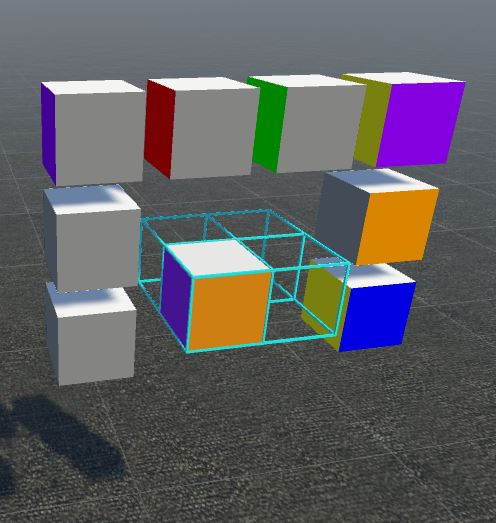
\includegraphics[width=0.5\textwidth]{vr_task_initialstate}
\caption{Initial state of the task: In the center - the solution space in light blue with the starting cube. Surrounding the solution space - the 9 remaining cubes to interact with. }
\label{fig:vr_task_initialstate}
\end{figure}

\newpage

The goal state of the task is achieved when all slots of the solution space are filled with a cube and all 6 faces of the resulting cuboid are colored differently but also unicolored each. The colors of the goal state displayed in Figure \ref{fig:vr_task_goalstate} are the following (not all colors can be seen because of the perspective):

\begin{center}
\textbf{front=orange, back=red, left=purple, right=blue, top=white, bottom=black}
\end{center}

\begin{figure}[h]
\centering
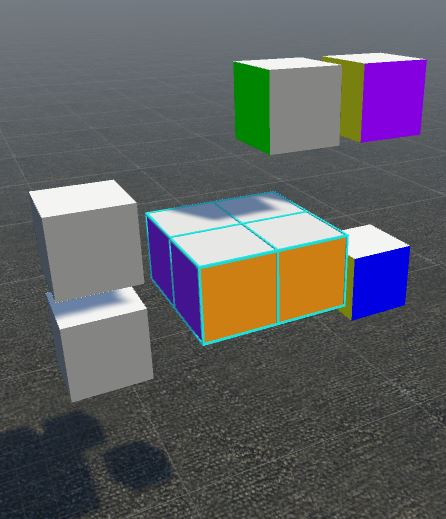
\includegraphics[width=0.5\textwidth]{vr_task_goalstate2_4}
\caption{Goal state of the task: All slots of the solution space are filled with a cube and all 6 faces of the resulting cuboid are differently colored, but also unicolored each. }
\label{fig:vr_task_goalstate}
\end{figure}

There are only 3 cubes that fit to achieve the goal state. Each of those 3 cubes fits exactly into one specific slot of the solution space. Those 3 cubes will be referred to as the "goal cubes". The remaining 6 cubes will be referred to as the "distractor cubes".

\subsection{Task rules} \label{sec:task_rules}
The most important rule of the task is that the cubes have to be put into the slots of the solution space in a certain sequence.
This sequence is shown in Figure \ref{fig:task_rules}). When participants see the task in front of them, the starting cube is always located in the left slot close to the participant (1). The second slot in the sequence - which is actually the first slot participants fill themselves - is the the slot behind the first slot (2). The third slot is the to the right of the starting cube (3). And the fourth slot is behind the third slot (4). When participants need to remove cubes, they have to do it in the reverse order. One example situation in which they need to remove cubes will be described in the following: when the second and third slot of the solution space have already been filled, but there exists no 4th cube to make the solution complete, participants first need to remove the cube from the 3rd slot. Optionally they can try to replace it with another cube to see if it leads to the solution. If they decide to keep the third cube removed, they can also remove the second cube. It is not allowed to remove the second cube as long as there still is a cube placed into the third slot. 

\begin{figure}[h]
\centering
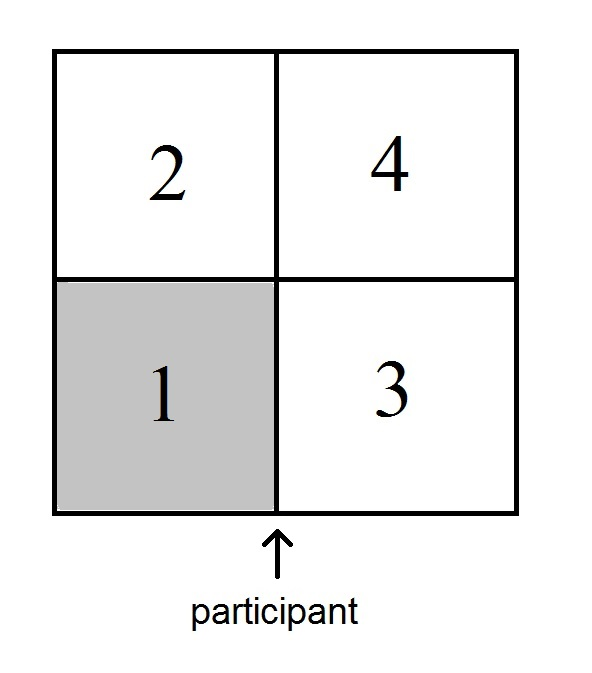
\includegraphics[width=0.5\textwidth]{task_rules}
\caption{Top down view of the task, showing the sequence in which cubes have to be but into the slots of the solution space from 1 to 4. }
\label{fig:task_rules}
\end{figure}

\subsection{Task theory}
An important aspect of the task design was to reduce the variations of how participants could solve the task. In this section the theories and main concepts of the task design will be explained in order to show that it suits well to perform controlled spatial problem solving experiments.

\subsubsection{Binary tree structure}
The main characteristic of the task is that there are several partial solutions to the problem because of the distractor cubes. Those partial solutions and the actual solution can be displayed in a binary tree. (see Figure \ref{fig:vr_tree}) The binary tree is representing the 4 paths which a participant may use in order to find the solution. The root node of the tree represents the initial state of the task showing the colors of starting cube in the solution space. Since the task was designed to have a binary tree structure there are always two options to put in a cube in a slot, following the given sequence. Therefore following two nodes represent the two options to place a second cube. The same applies to the next level of the tree. The solution space has been rotated for each node in a way that the relevant colors are visible. The bottom nodes show the possible end state of each path. It can be seen that only the right path leads to the goal state.

\begin{figure}[h]
\centering
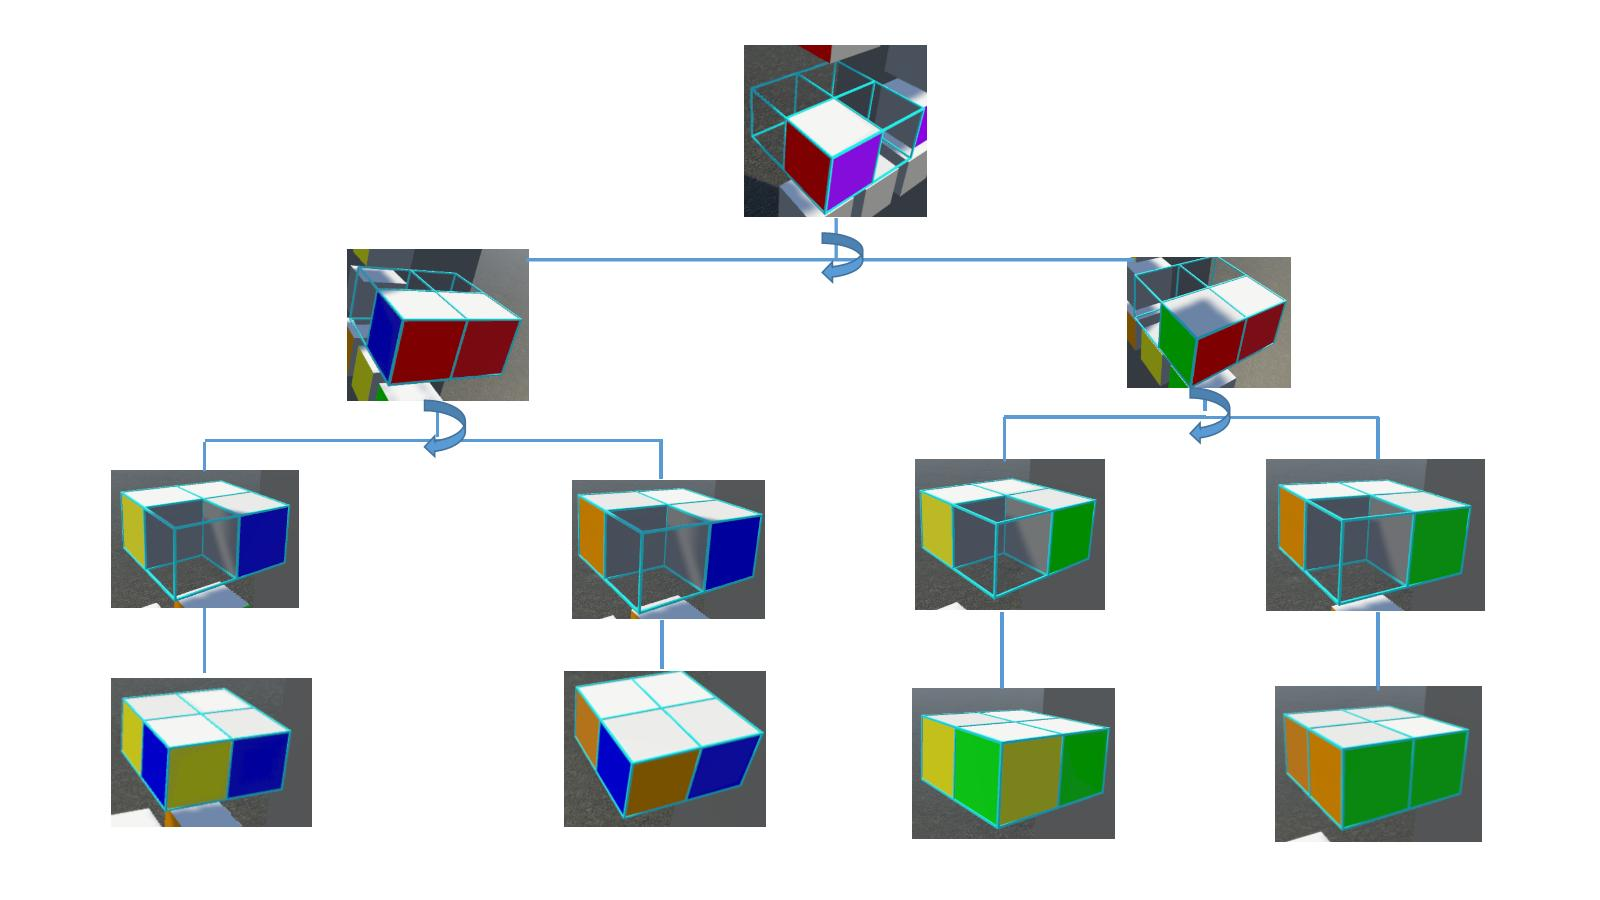
\includegraphics[width=1.0\textwidth]{vr_tree}
\caption{Binary tree structure of the different solution paths of the task.}
\label{fig:vr_tree}
\end{figure}

Since distractor cubes are colored in a way that they appear to be part of the solution, participants can not instantly find the solution (unless they are lucky). The idea of the task is that participants have to apply a try and error strategy, but in a very systematic way. In order direct the participants towards this systematic try and error strategy, they receive the instructions to follow the sequence in which cubes have to be put into (and removed from) the solution space (as described in Section \ref{sec:task_rules}). As it can be seen in Figure \ref{fig:vr_tree} there are 4 possible paths in the tree to fill the solution space. But only one path leads to the correct solution and therefore there is a 25\% chance to instantly solve the task - assuming participants always stick to the sequence rules. In the worst case they need to try all 4 paths to find the solution. This also means that by design each task trial should be possible to be solved within a certain amount of time, which is beneficial to compare the time performances between the individuals and groups of two. 

Besides the predictable solution time, the tree structure also allows to precisely quantify the actual error of participants. The amount of paths within the tree participants need to try is random and therefore not controlled. This means the actual performance is both flawless when participants need to try only 1 or all 4 paths of the tree. An actual error occurs only when participants repeatedly try the same path of the tree. Such an error can be ascribed to the working memory since in this case participants clearly forgot that they tried the same path before.

\subsubsection{Simplifications}
One simplification of the task was to have only one solution. This has been achieved by designing the task in a way that there are only the 3 goal cubes which are part of the solution. None of the goal cubes can be exchanged by another cube so that for each trial all participants have the exact same goal state.

Furthermore some of the cube colors always have the same meaning and therefore support the participants in finding the right orientation for each cube within the solution space. White always indicated the top face of a cube in the solution space, black always indicated the bottom face of a cube in the solution space. Thus, participants only need to find the correct orientation of a cube in the vertical rotation axis. The gray faces always indicate the faces which point into the center of the solution space and have a similar function because they help to correctly orient the cubes within the solution space.

\subsubsection{Trials}
Both in the single and group condition participants have to solve 20 trials of the task. The benefit of the task design is that 20 different instances of the task can be generated. And the instances only differ in colors as described in Section \ref{sec:task_components} Thus the complexity or difficulty is the same for each trial and at the same time participants can not learn the position or the colors of cubes in the initial state, since they change from trial to trial. For each participant we use a randomized order of the 20 trials, but the pool of trials is the same.

Another aspect of the repetitive execution of the same task is that participants are supposed to improve over time, because they are expected to understand the tree like structure of the task and therefore get better at avoiding errors (trying the same path more than once). This aspect of the task design is only mentioned for completeness, but will not be further discussed in this study.


\subsubsection{Summary}
Both the binary tree structure of the task and the simplifications reduce its complexity so that it is more controlled. This makes it is easier to analyze the performance of participants. The task design is intended to be suitable for different kinds of research questions in the field spacial problem solving. In this work the focus is the comparison between the performances of individuals and groups of two.
\newpage
\section{Methods}

\subsection{Participants}
Twenty participants(10 female, 10 male; all right-handed) from the local university community participated in the experiment. Their age ranged from 21 to 32 years. All participants were naive to the purpose of the experiment and had normal or corrected-to-normal vision. The experiment was approved by the ethics committee of the University of T\"ubingen, and was performed in accordance with the Declaration of Helsinki. Participants gave written informed consent prior to the experiment and were compensated with 8 Euro per hour for their participation. 

\subsection{Apparatus}
The virtual environment was displayed in stereo using an HTC Vive head-mounted-display (HMD) with a resolution of 1080 x 1200 pixels per eye (2160 x 1200 pixels combined). Inter-pupillary distance was measured with a pupilometer and set accoringly on the HTC Vive for each participant. Audio was recorded with a microphone plugged into the integrated audio input of the HTC Vive. Participants were standing during the whole experiment and viewed their virtual task in front of them.

Participants were run in an individual and a collaborative condition in which two participants worked together. Therefore the apparatus consisted of two HTC Vives of which each was connected to its own computer. The computers had the same hardware configuration. In the individual condition participants were run in their own virtual environment solving the task alone. In the collaborative condition two participants were run in a shared virtual environment solving the task together (see Figure \ref{fig:procedure_real_two} and \ref{fig:procedure_vr_two}). The synchronization between the two computers in the collaborative condition was done via UDP. Therefore participants could collaborate in real time with very little to no delay.

The virtual task consists of cubes and cube slots. The cubes can be picked up by moving the controller into a cube and pressing and holding the trigger button of the controller (there is both no collision between cubes and between cubes and the controller). When a cube is picked up it can be moved and rotated freely with the controller. When the cube is moved to the solution space it  automatically aligns ("snaps in") with the next closest cube slot.

\begin{figure}[h]
\centering
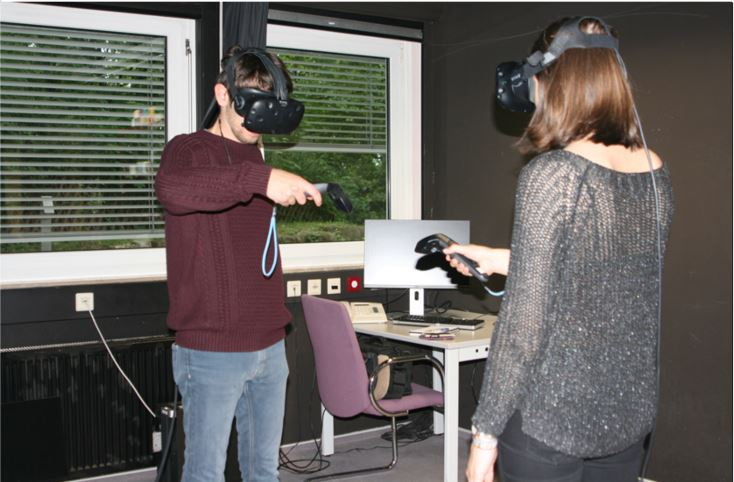
\includegraphics[width=0.75\textwidth]{procedure_real_two}
\caption{Two participants solving the task together in the collaborative condition.} \label{fig:procedure_real_two}
\end{figure}

\begin{figure}[h]
\centering
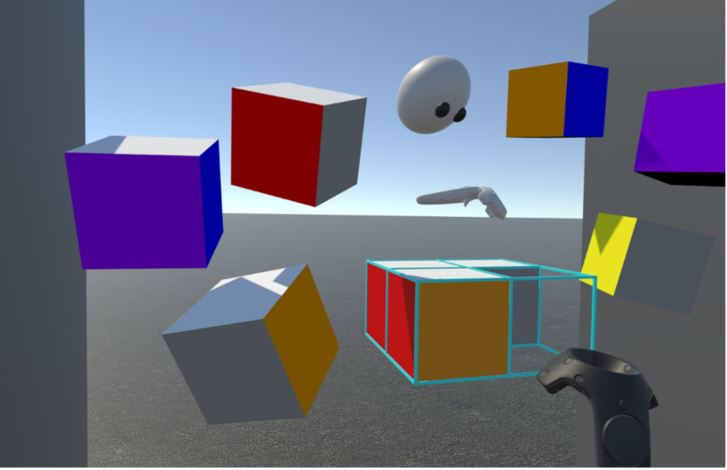
\includegraphics[width=0.75\textwidth]{procedure_vr_two}
\caption{Virtual reality scene of two participants in the collaborative condition. The gray sphere represents the head of the other participant. The gray controller is the controller of the other participant.}
\label{fig:procedure_vr_two}
\end{figure}

\newpage

\subsection{Procedure}
Participants were invited as a group of two people and did not know each other. In one group session the two participants solved the task on their own in a separate virtual environment and together in the same virtual environment. The sequence of single and collaborative condition was counter balanced among all groups. In both the single and collaborative condition participants solved 20 tasks of which all had the same design as described above and differed only in color. In the single condition participants viewed the task always from the same perspective, which means that the starting cube was always placed at the same position in the solution space.
In the collaborative condition we rotated the solution space after 10 trials, which means the starting cube is on one participant's side for the first 10 trials and on the other participant's side for the remaining 10 trials. 

The detailed procedure for the single condition will be explained in the following:
After having read the instructions of the task participants also received a verbal instruction by the experimenter. Before the actual 20 trials began participants had to solve 4 training trials in order to verify that the participant understood the task and the way it has to be solved. It was emphasized that it is important to always stick to the sequence of putting in and removing cubes as described above. Furthermore participants could experience that the starting cube can not be removed and is the only cube in the experiment that collides with the other cubes (that was important to prevent other cubes from overlapping with the starting cube). Participants could also get used to the fact that the top color is always white and the bottom color is always black and that gray always faces to the inside of the solution space. The training trials could be started by the participant by holding a controller button for 2 seconds. When they started the training they saw the solution space surrounded by the 9 cubes which are all in reaching distance. They also saw the starting cube already being placed into the solution space. Above the task participants could see in which trial they currently are. In this case they would see "Training 1/4". Once they have finished a trial they can proceed with the next trial by pressing the controller button again for 2 seconds. 

Before the actual 20 trials started the experimenter repeated the most important instructions. Participants should try to solve the task as quickly and as accurately as possible. Furthermore they were not allowed to move around the problem space and should stay mostly stationary in their position with only a few steps to the sides allowed.
After the 4 training trials participants could start the actual trials as soon as they were ready by clicking a controller button again for 2 seconds. For the actual trial the experimenter would emphasize that participants should always make sure their solution is correct before proceeding with the next task. In case participants did not correctly solve a task and still proceed with the next task the experimenter took notes in order to exclude the trial from the analysis.

The procedure for the collaborative solving of the task was mostly the same. The only difference was that just one participant was able to skip to the next trial and therefore the instructions were that participants had to agree on when to proceed with the next task.

%what needs to go in here is:

%instructions that were given to the participants
%training phase (how many trials...)
%counterbalance single / multi (counterbalanced - 10 each side)

\newpage
\section{Results}
Data analysis was done by applying linear mixed models with the Kenward-Rodger degrees of freedom approximation. The random factors were the group number (= an individual number assigned to each group in the group condition), participant number (= an individual number assigned to each individual participant in the single condition) and the number of players(= either one or two). The only fixed factor was the number of players. 

 Although much more data has been recorded during the experiment this section will only cover the most relevant results that suit best to compare the performances of the single vs the group condition. 
 
 All data was automatically recorded from the time participants pressed the controller button to start the task to when they pressed the button again in order to skip to the next task. The data was based on the controller trajectories, rotations and user input.  In the following the term "task duration" will be used to describe the duration in which data was recorded for an individual task.

\subsection{Time to complete}
The time to complete is the average of all task durations.  Figure \ref{fig:results_duration} shows that the groups were much faster with an average of around 50 seconds compared to single participants with an average of around 80 seconds. The output of the linear mixed model was F:(1,18.99) = 52.049, p < 0.001.

\begin{figure}[h]
\centering
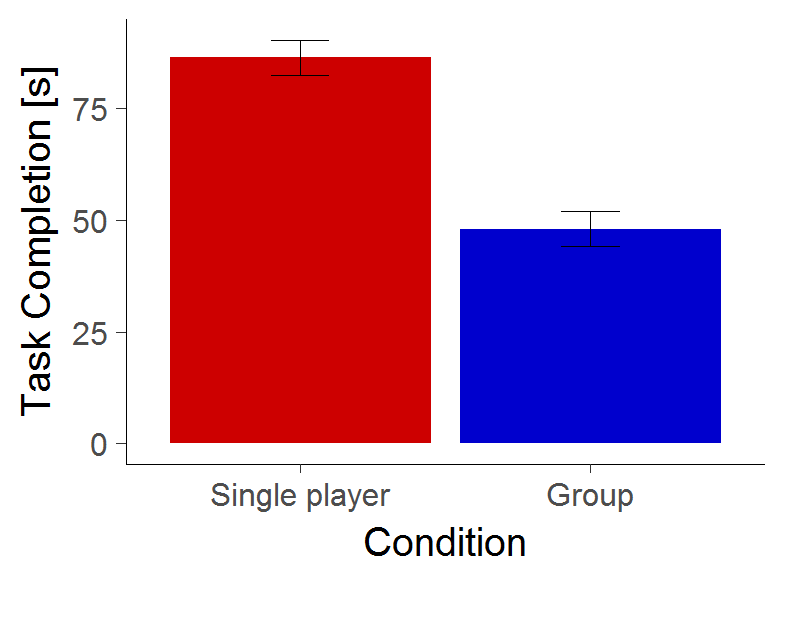
\includegraphics[width=0.5\textwidth]{results_duration}
\caption{Average time to complete in single and group condition.} \label{fig:results_duration}
\end{figure}

\subsection{Rotation sum of cubes}
The rotation sum of cubes is the sum of rotations made by one participant during the task duration. In the group condition we summed up the rotations of both group members first and calculated the averages over the group sums. Figure \ref{fig:results_rotations} shows that the average rotation sum for groups with an average of 5000 degrees was significantly lower compared to single participants with an average of 8000 degrees. For the rotation sum a the smaller value indicates the better performance because the less a participant rotates a cube the more confident and efficient the participant is expected to be at solving the task. The output of the linear mixed model was F:(1,18.99) = 12.164, p < 0.01.

\begin{figure}[h]
\centering
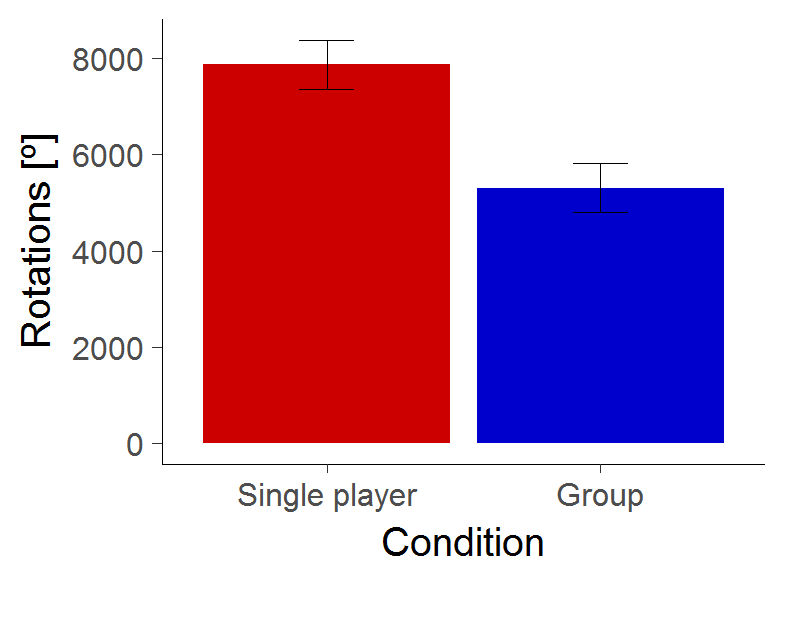
\includegraphics[width=0.5\textwidth]{results_rotations}
\caption{Average sum of rotations in degrees in single and group condition.}
\label{fig:results_rotations}
\end{figure}

\subsection{Number of cube snap-outs}
The number of cube snap-outs is the number of how many times a participant took a cube back out from the problem space during the task duration. Figure \ref{fig:results_snap_outs} shows that groups needed much less snap-outs with an average of 2.1 snap-outs compared to single participants with an average of 4.5 snap-outs. 
Snap-outs can be categorized in two classes: "necessary" and "unnecessary" snap-outs. Necessary snap-outs are the ones which are part of the task design which means participants are supposed to try certain solution paths and if a path was not successful they need to snap-out some cubes and snap-in new ones until they successfully finish the task. It is possible though that participants try the same solution path more than one time and therefore have to do unnecessary snap-outs. For the number of cube snap-outs a smaller value indicates the better performance, because it means that less unnecessary snap-out were made. The average of necessary snap-outs is expected to be equally distributed with an expectancy value of 2.0. In other words scoring an average of 2.0 snap-outs is an indicator of almost "perfect" performance. In the group condition the performance is very close to perfect with an average od 2.1 snap-outs.
The output of the linear mixed model was F:(1,18.99)=22.112, p < 0.001.

\begin{figure}[h]
\centering
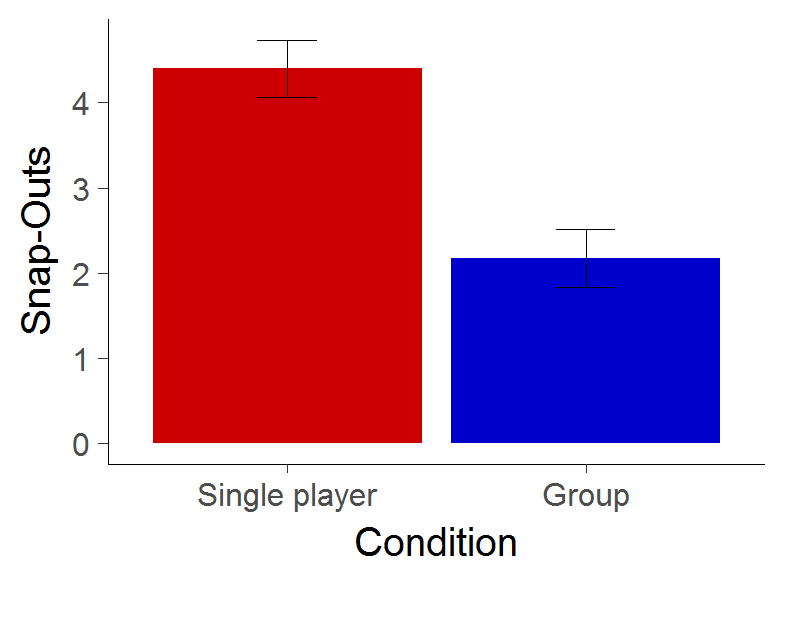
\includegraphics[width=0.5\textwidth]{results_snap_outs}
\caption{Average number of cube snap-outs in single and group condition.}
\label{fig:results_snap_outs}
\end{figure}

\newpage
\clearpage
\section{Discussion}\label{discussion}

Designing a task for spatial problem solving is quite complex and many factors have to be taken into consideration. In order to achieve meaningful results from experiments that are based on such a task, it is important that the task is very controlled. When it comes to comparing individuals and groups in problem solving it must be made sure that the task can be executed in a similar manner both in the individual and group condition. We decided to position participants in the individual condition in front of the task having the starting cube on their side of the solution space. In the group condition we positioned the two participants on two sides of the problem space facing each other. Therefore only one participant in the group condition can have the same position as in the individual condition. The other participant stands on the other side of the problem space having a completely different perspective of the problem. It is intended that participants have different perspectives of the problem in the group condition, because perspective is a relevant factor in spatial problem solving - especially when it comes to collaboration. \cite{Amorim2003} In natural settings two or more people working on the same problem usually do not have the same perspective and therefore have a cost in communicating the differences in perspective and must to try create a shared representation (\cite{Roschelle1995} and \cite{Frankenstein2012}) of the current state of the problem on which they are working together. In the collaborative condition participants have the same costs of communicating the differences in perspective. Nevertheless, it could be found that the beneficial aspects of having two different perspectives and being able to work together proved to prevail the costs of communication and shared representation. This is assumed to be the main reason why groups performed much better than individuals.

Another benefit of working together on the task, was that participants were able to simultaneously work on different sub processes of the problem. While one participant identifies the required colors for the next slot, the other participant can already start searching in the remaining cubes and maybe sort them into relevant or irrelevant cubes based on the current colors that are already part of the solution space.

Since the task was very controlled and did not leave too many options of how to transition from the initial state to the goal state, the question arises if the group condition would have also performed this much better if there would have been no information about the sequence of putting the cubes into the solution space. This could be easily tested in a follow up study, in which the information about the sequence is omitted. All other aspects of the experiment could remain the same.

In another follow up study the advantage of virtual reality to put both participants in the same position could be used in order to find out how much of an effect a shared perspective has on the performance. It is difficult thought to have two people interact from the exact same virtual location with a virtual environment since collisions and conflicts in actions are more likely to occur. This variation also obviously can not occur in a real live scenario at all, but comparing that variation to the results presented in the current study may give interesting insights on how relevant perspective is for collaborative spacial problem solving.

Furthermore the combination of virtual reality with eye tracking could help to better understand the cognitive processes involved in collaborative spatial problem solving when it comes to action planning and execution. 
\newpage
\section{Conclusion}\label{conclusion}
Finally, it can be said that the approach presented in this study can be considered as a basis for future research to further investigate the relevant cognitive processes involved in collaborative spatial problem solving. This study was intentionally designed to be very controlled and therefore does not compare to any application of real life problem solving. The goal was to design a task that allows to quantify performance in spacial problem solving tasks. Also the study proved virtual reality to be a well suited method of research for the field of collaborative spatial problem solving. The main finding was that groups perform significantly better than individuals in the designed spatial problem solving task. Further research will have to show if the same applies for more complex variations of the task and how important factors like perspective and communication are.

\onecolumn
% einfacher Zeilenabstand
\singlespacing
% Literaturliste soll im Inhaltsverzeichnis auftauchen
\newpage
\addcontentsline{toc}{section}{Bibliography}
% Literaturverzeichnis anzeigen
\renewcommand\refname{Bibliography}
\bibliographystyle{plainnat}
\bibliography{Hauptdatei}

%% Index soll Stichwortverzeichnis heissen
% \newpage
% % Stichwortverzeichnis soll im Inhaltsverzeichnis auftauchen
% \addcontentsline{toc}{section}{Stichwortverzeichnis}
% \renewcommand{\indexname}{Stichwortverzeichnis}
% % Stichwortverzeichnis endgueltig anzeigen
% \printindex

\onehalfspacing
% evtl. Anhang

% Eidesstattliche Erklärung
\section*{}
\thispagestyle{empty}

\begin{verbatim}

\end{verbatim}

\begin{LARGE}Eidesstattliche Erklärung zur Masterarbeit\end{LARGE}
\begin{verbatim}


\end{verbatim}
Ich versichere, die von mir vorgelegte Arbeit selbstständig verfasst zu haben. Alle Stellen, die wörtlich oder sinngemäß aus veröffentlichten oder nicht veröffentlichten Arbeiten anderer entnommen sind, habe ich als entnommen kenntlich gemacht. Sämtliche Quellen und Hilfsmittel, die ich für die Arbeit benutzt habe, sind angegeben. Die Arbeit hat mit gleichem Inhalt bzw. in wesentlichen Teilen noch keiner anderen Prüfungsbehörde vorgelegen.



\begin{displaymath}
% use packages: array
\begin{array}{ll}
Unterschrift:~~~~~~~~~~~~~~~~~~~~~~~~~~~~~~~~~~~~~~~~~~
& Ort, Datum:~~~~~~~~~~~~~~~~~~~~~~~~~~~~~~~~~~~~~~~~~~
\end{array}
\end{displaymath}


\end{document}